\clearpage
%\newpage
\section{Preparation}
The preparation phase provides basic information about a target application's performance
behaviors. 
Such information can be obtained by many performance tools.
We currently accept performance data generated by HPCToolkit and GNU gprof.

\subsection{Using HPCToolkit}
%The HPCToolkit~\cite{hpctoolkit} is developed at the Rice University to get
%performance metrics of the target application. 
The HPCToolkit~\cite{hpctoolkit}, developed at the Rice University, is an open source profile-based
performance analysis tool sampling the executions of optimized applications. No code
instrumentation is needed to use HPCToolkit. But debugging information (by compiling with
the -g option if GCC is used) in the binary executables is needed for the tool to
associate performance metrics with source language constructs.

After installation, a typical session of using HPCToolkit is given below:
{\mySmallFontSize
\begin{verbatim}
% Prepare the executable with debugging information
gcc -g smg2000.c -o smg2000 

% Sample one or more events for the execution, use wall clock here
hpcrun -e WALLCLK -- ./smg2000 -n 120 120 120 -d 3

% Convert the profiling result into a XML format
hpcproftt -p -D /home/liao6/svnrepos/benchmarks/smg2000 ./smg2000 \
  smg2000.WALLCLK.tux268.llnl.gov.10676.0x0 > result.xml

\end{verbatim}
}

\fixme{TODO: update the text when the latest release of HPCToolkit works
on 32-bit platforms}

%A SMG2000~\cite{BrownSemicoarsening2000} (Semicoarsening Multigrid Solver) benchmark from the ASCI Purple
%benchmark suite is chosen to exemplify the use of this system.

Fig.~\ref{fig:hpctoolkitSmg2000} shows the profiling results of SMG2000
using HPCToolkit. 
A statement in a loop takes more than 46\% execution time, which makes the
loop dominant, most expensive loop of the entire program.
\begin{figure}[htbp]  
	\centering
		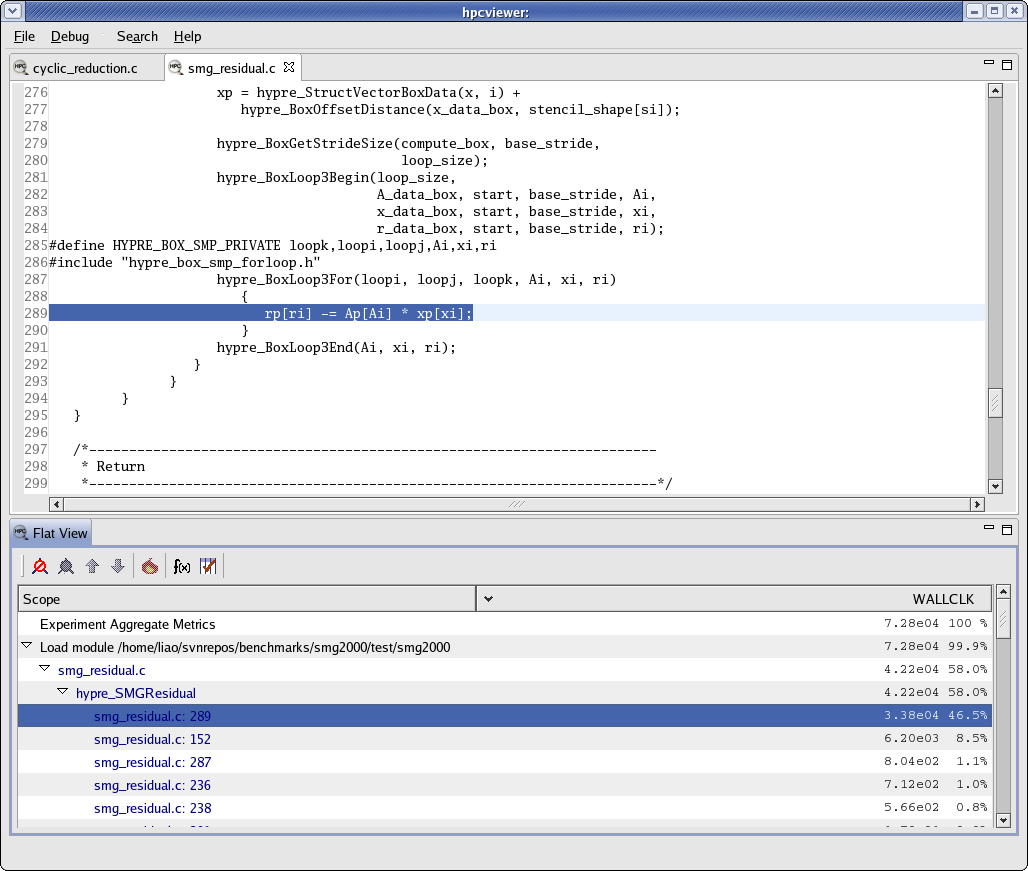
\includegraphics[width=0.9\textwidth]{hpctoolkit-smg2000.png}
	\caption{Profiling results of SMG2000 using HPCToolkit}
	\label{fig:hpctoolkitSmg2000}
\end{figure}

\subsection{Using gprof}


